\documentclass[a4paper,12pt,twoside]{book}
\usepackage{graphicx}
\usepackage{fancyhdr}
\usepackage[font = scriptsize, bf]{caption}
\usepackage[english]{babel}
\usepackage[utf8x]{inputenc}
\usepackage[parfill]{parskip}
\usepackage{amsmath, amssymb}
\usepackage{moreverb}
\usepackage{algorithm} %
\usepackage{algpseudocode}
\usepackage[usenames,dvipsnames]{color}
\usepackage[swapnames]{frontespizio}
\usepackage{url}
\usepackage{setspace}
\usepackage{eqparbox,array}
\usepackage{siunitx}
\usepackage{subfigure} 
\usepackage{wrapfig}
\usepackage{amsthm}
\usepackage{eurosym}

\renewcommand{\algorithmiccomment}[1]{  //\emph{\textcolor{Gray}{#1}}}


% Sistema i margini per lasciare più spazio di rilegatura
\addtolength{\oddsidemargin}{+1,3cm} 
\addtolength{\evensidemargin}{-1,3cm} 
\onehalfspacing

% Imposta lo stile della prima pagina del capitolo
\fancypagestyle{plain} {
    \fancyhead{}
    \fancyfoot[LE,RO]{\thepage}
    \renewcommand{\headrulewidth}{0pt}
}

\DeclareMathOperator*{\argmax}{arg\,max}
\newcommand{\compInterfacciaDB}{Data Interface}
\newcommand{\compLoader}{Loader}
\newcommand{\compMatrix}{Matrix Creator}
\newcommand{\compTermsSel}{Terms Selector}
\newcommand{\compPosition}{Position Calculator}
\newcommand{\compClustering}{Clustering Component}
\newcommand{\compEvolution}{Evolution Discoverer}

\hyphenation{ti-me-win-dow}

\graphicspath{{./Immagini/}}


\begin{document}

% frontespizio
\begin{frontespizio}
  \Istituzione{University of Bari ``Aldo Moro''}
  \Logo[3.5cm]{Immagini/logo_uni.jpeg}
  \Divisione{Department of Computer Science}
  \Scuola{Master's Degree in Computer Science}
  \Titolo{Analysis of the state of the art on using natural interfaces to improve the user experience (UX) in the financial field}
  \Sottotitolo{AIINLP}
  \NCandidato{Student}
  \Candidato{Christopher Piemonte}
  \NRelatore{Professor}{Professors}
  \Relatore{Giovanni Semeraro}
  \Relatore{Fedelucio Narducci}
  \Piede{Academic year 2016-2017}
\end{frontespizio}

% \IfFileExists{Tesi-frn.pdf}{}{%
% 	\immediate\write18{pdflatex Tesi-frn}
% }

\IfFileExists{\jobname-frn.pdf}{}{%
\immediate\write18{pdflatex \jobname-frn}}

\pagestyle{fancy}
\fancyfoot{}
\fancyfoot[LE,RO]{\thepage}
\fancyhead{}
\renewcommand{\headrulewidth}{0pt}
\headheight = 15pt
\frontmatter

% indice
\tableofcontents
\afterpage{\null\newpage}


\frontmatter	
\mainmatter

% Imposta lo stile di intestazione e piè di pagina dei capitoli
\fancyfoot{}
\fancyhead{}
\fancyhead[LE,RO]{\slshape \leftmark}
\fancyfoot[LE,RO]{\thepage}
\renewcommand{\headrulewidth}{1pt}
\renewcommand{\chaptermark}[1]{%
\markboth{\thechapter.\ #1}{}}


% !TEX encoding = UTF-8
% !TEX TS-program = pdflatex
% !TEX root = ../Tesi.tex
% !TEX spellcheck = it-IT

%*******************************************************
% Introduzione
%*******************************************************
\cleardoublepage
\chapter*{Introduction}

Lo scopo di questo documento è di fornire una panoramica dello stato dell’arte nell’area della modellazione utente, analizzando la letteratura di riferimento, enfatizzando gli elementi caratterizzanti del progetto di ricerca rispetto allo stato dell’arte e sottolineando le analogie con alcune metodologie già presentate in letteratura.

Seguendo il titolo del progetto di ricerca, si è deciso di suddividere il rapporto tecnico in tre sezioni: nella prima saranno analizzati i principali lavori a stato dell’arte nell’area dello user modeling, fornendo una panoramica storica dell’area di ricerca e mostrando le principali tecniche per l’acquisizione dati e la modellazione utente. Successivamente si entrerà nel merito delle possibili sorgenti dati cui attingere per la costruzione dei modelli utente e si fornirà un’analisi critica delle stesse.

Nella seconda parte l’attenzione sarà focalizzata sui meccanismi per la rappresentazione semantica dell’informazione: in questo caso si introdurranno i concetti di base dell’area fornendo una panoramica sulle tecniche di semantic natural language processing e sulle tecniche a stato dell’arte per la rappresentazione dei profili, fornendo anche una serie di riferimenti su lavori già presentati in letteratura. Nell’ultima parte, infine, si studierà il tema della modellazione olistica dell’individuo, analizzando metodologie a stato dell’arte per l’aggregazione, il riuso e la mediazione di modelli utente. Infine si concluderà il report illustrando le principali soluzioni tecnologico-architetturali per la modellazione utente ed infine analizzando criticamente quanto presentato, enfatizzando gli elementi caratterizzanti del progetto rispetto allo stato dell’arte attuale.


\chapter{Background}
\label{cap:capitolo1}
% !TEX encoding = UTF-8
% !TEX TS-program = pdflatex
% !TEX root = ../Tesi.tex

%************************************************

%************************************************

Speech or text interaction between human beings and computers is gaining more and more popularity nowadays. People want to communicate with computers in the same manner as they communicate with other human beings. One of the main tools used for analyzing speech and providing human-like answers is Natural Language Processing (NLP). In order to provide suitable responses based on phrases or keywords taken from questions as well as to keep the communication continuous, there is a need to create a dialogue system or program, which is often called a chatbot or a chatterbot. The chatbot is a computer program that has the ability to communicate with people by providing answers to questions and holding the conversation using Natural Language Processing. People input the natural language speech or text, while the program should provide the most suitable intelligent response in the form of text or speech. As long as the communication continues, this process is repeated.

% 
% * <siciliani.lu@gmail.com> 2018-04-06T15:09:35.037Z:
% 
% > is being repeated
% is repeated
% 
% ^.
% * <siciliani.lu@gmail.com> 2018-04-06T15:08:49.012Z:
% 
% > an ability
% the ability
% 
% ^.
% * <siciliani.lu@gmail.com> 2018-04-06T15:07:15.934Z:
% 
% > the human and the computer 
% human beings and computers
% 
% ^.


\section{User eXperience}

This chapter gives an overview of UX, distinguishes it from the concept of experience and presents the current research status, definitions and viewpoints of UX. Definition, in theory, is easy since the ISO 9241-210:2010 standard defines UX as follows: \textit{"A person's perceptions and responses that result from the use and/or anticipated use of a product, system or service."} \cite{ergonomics2011}. Apparently the definition and meaning are not that easy since UX is an umbrella term \cite{instone2005}. In some studies UX is regarded as a synonym of UI (User Interface), whereas in other studies it might be usability or anything vaguely related to users and technology. The following is a selection of UX views from various sources:

% * <siciliani.lu@gmail.com> 2018-04-06T15:17:30.914Z:
% 
% > are
% "is" (non si riferisce a "selection"?)
% 
% ^.
% * <siciliani.lu@gmail.com> 2018-04-06T15:11:44.975Z:
% 
% > some
% La renderei più formale. Direi qualcosa tipo "In some studies UX is regarded as a synonym of UI,  whereas...."
% oppure "UX  is sometimes seen as a synonym of UI, ..."
% 
% ^.
% * <siciliani.lu@gmail.com> 2018-04-06T15:11:24.270Z:
% 
% > equal with
% equal to
% 
% ^.
% * <siciliani.lu@gmail.com> 2018-04-06T15:10:10.129Z:
% 
% > from experiences
% Forse meglio: "distinguishes it from the concept of experience" ?
% 
% ^.

\begin{itemize}
\item UX is dependent on the subject, object, and interaction between these two \cite{luojus2010}.
\item No amount of professionalism in UX can substitute for our being personally involved \cite{alben1997}.
\item UX varies between situations and may change over time \cite{hassenzahl2003}.
\end{itemize}

All the above statements strongly emphasize the role of the user and his or her demographics and abilities as well as the current context of the user.

As Hassenzahl stated \textit{"There is no guarantee that users will actually perceive and appreciate the product the way designers wanted it to be perceived and appreciated"} \cite{hassenzahl2003}.

So what is the the difference between experience or user experience? 

Roto has taken a similar approach in her dissertation when she separates UX from experiences: \textit{“I claim that user experience is a special case of experience, where the person can use a system, with or without a purpose. Using means that the user not only senses the system, but also has the opportunity to manipulate or control the system. The system is a product, object, or a set of them; service systems often involve a human being such as a librarian. If there is no system at all, or if the person cannot control the system, we should use the term experience instead of user experience.”} \cite{roto2006}.



\section{Conversational User Interfaces}

In the Oxford English Dictionary a conversation is defined as a talk, especially an informal one, between two or more people, in which news and ideas are exchanged. This definition suggests that initiative belongs to both sides of the conversation, Radlinski and Craswell \cite{radlinski2017} calls this mixed initiative. Even though it is in the most recent years that conversational interfaces have gained widespread usage, they have been around for many years. Starting in the 60's with text-based dialogue systems for questions and answers, and chatbots that simulated natural conversations \cite{mctear2016}. Voice-based systems began to appear in the late 80's and spoken dialog technology became a key area of research within the speech and language communities \cite{mctear2016}. At the same time Voice User Interface (VUI) started to emerge and social robots that could mimic human expressions were developed. These human-like systems were developed in order to provide a more engaging interaction \cite{mctear2016}. According to Radlinski and Craswell \cite{radlinski2017} a conversational system is an information retrieval system that permits a mixed-initiative between an agent and user, where the agent's actions are based on the conversation, using both short and long term knowledge of the user. They further discuss that a conversational system needs to have at least five properties:


\begin{itemize}
\item \textit{User Revealment} - the system helps the user to express their needs.
\item \textit{System Revealment} - the system is clear with its capabilities to form user expectation of the system.
\item \textit{Mixed Initiative} - both system and user can take initiative for conversation.
\item Memory - the user can reference past statements and the system understands.
\item \textit{Set Retrieval} - The system can reason about the utility of sets of complementary items.
\end{itemize}


\subsection{Voice User Interfaces}

A VUI is what a user interacts with when communicating with a device or system using their voice \cite{cohen2004, mctear2016}. Even though it is in the most recent years that speech recognition technology has gained wide spread usage, it has been around for almost a century \cite{cohen2004}. The first success story was actually a children’s toy, called Radio Rex in the beginning of the 20th century. Radio Rex could react and run upon its owner's call \cite{cohen2004}. Today the technology has come a long way, and VUIs are often coupled with Intelligent Personal Assistants (IPA). An \textbf{IPA} is a software agent that can perform tasks or services for an individual. These tasks or services are based on user input, location awareness and the ability to access information from a variety of online sources. The user often interacts with an IPA through a VUI and today companies such as Google, Apple, Microsoft and Amazon have developed their own IPAs based on VUIs.
% * <siciliani.lu@gmail.com> 2018-04-06T15:42:26.487Z:
% 
% > Even though it is in the most recent years that speech recognition technology has gained wide spread usage, it has been around for almost a century
% Nel paragrafo precedente c'è una frase quasi identica, ma senza citazione.
% 
% ^.

\section{Chatbots}
Chatbots produce natural responses to human user text inputs \cite{mctear2016}. Chatbots are developed to trick the user into believing that they are conversing with another human \cite{mctear2016}. To date most chatbots have been text based, but as new speech recognition technology has evolved more chatbots make use of speech as input and output. It is most common that the chatbot responds to user input rather then being the initiator of the conversation \cite{mctear2016}. Chatbots were first developed in the 60's. Weizenbaum \cite{weizenbaum1966} developed a system called ELIZA, which simulates a psychotherapist. ELIZA was mainly created to demonstrate the superficiality of communication between man and machine \cite{mctear2016}. Today chatbots are increasingly being used in areas such as education, information retrieval, business and e-commerce.
% * <siciliani.lu@gmail.com> 2018-04-06T15:43:23.338Z:
% 
% > user input
% to the user input
% 
% ^.

According to McTear et al. \cite{mctear2016} a conversational chatbot interface should operate as follows: 

\begin{itemize}
\item Recognize the text that was sent by the user.
\item Interpret the words and discover what the user meant with this input.
\item Formulate a response, or if the message was unclear, interact with the user to find clarification.
\item Construct the response, which may be in the form of words or accompanied by visual and other types of information.
\item Display the response.
\end{itemize}


\begin{figure}[htb]
	\centering
	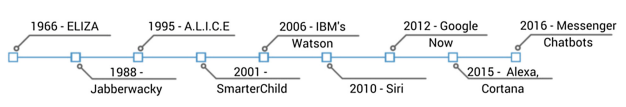
\includegraphics[width = 100mm]{chatbot-history}
	\caption{History of chatbots.}
	\label{chatbot-history}
\end{figure}

% \subsection{Rule-Based Bots}

% \subsection{AI Bots}






\subsubsection{Messenger Bots}
In April 2016, Facebook released their chatbot feature in Messenger. The main purpose was to increase people's experience with the platform and to let businesses reach out to their customers in a completely new way \cite{messenger}. To make it easier for developers and designers to build beautiful and consistent messenger bots that allows for a unified experience, Facebook released design guidelines to follow \cite{messenger_guidelines}. The messenger bot design guidelines are organized under three main headings:

\paragraph{Design Principles}
Facebook \cite{messenger_guidelines} suggest that bots should be brief. Since most people use messenger on their phone, interruptions should be expected. The easiest way to address this according to Facebook is to keep interactions short and concise. When that is not possible, developers and designers should consider how to maintain and reestablish context. Facebook \cite{messenger_guidelines} also advice to avoid modality; modality can create confusion and frustration for the users if they are interrupted in the middle of a task. Furthermore, conversations and graphical user interfaces (GUIs) should be mixed in the bots; Facebook offers a range of components, and these should be used depending on the bots functionalities and capabilities. It is also important to observe conversational norms and Facebook highlights the relevance to be deliberate about language, editorial voice, length of messages, and even speed of response. Embracing structure is also important when building a messenger bot. Making use of buttons, quick replies, and the persistent menu to structure user interactions while clearly communicating expectations. Moreover, Facebooks highlights the importance of developing a bot that notifies with care, fails gracefully, and is predictable in its interactions.

\paragraph{Language \& Editorial Voice}
Because bot interactions take place on Messenger, a messaging platform, the words used are important in explaining the experience a bot provides and why people should use it. Thus, Facebook suggest methods for writing interactions and best practices \cite{messenger_guidelines}. As writing best practices they suggest that it is important to preserve a voice, set user expectations, and to provide context. The bots voice or way of communication reflects its personality; it is essential to be consistent with it, in a tone that feels natural and human. It should also be easy for users to know what the bot can, or can not do, in order to set the correct user expectations. Further, bots should be as descriptive as possible to communicate core functionality; to build an understanding of the experience the bot creates, content should guide users every step of the way. Facebook also suggest designers and developers to design conversations before launching a chatbot. This can be done by starting to build a library of prompts and responses. According to them it is important to think about the goals and possible outcomes of a conversation, they also emphasis on creating a list of keywords to really get an overview of terms associated with the bot. Facebook also believe that mapping out interactions is a good idea, mapping gives a good overview of the tasks, expectations and contexts to establish with the bot. User responses can later be used to expand functionalities and capabilities \cite{messenger_guidelines}.

\paragraph{Tips for Sounding More Conversational}
In the end of their guidelines, Facebook gives tips on how to sound more conversational in writing. They emphasize on the importance of the chatbots style of writing; it has to converse in a way that its utility is not misrepresented or core capabilities are misunderstood. Furthermore, Facebook state that a conversational tone should support an experience, not define it \cite{messenger_guidelines}. They give some simple suggestions in how to implement a conversational tone in a chatbot by using an active voice, contractions of words, write in first and second person, to be careful with grammar and punctuation, and lastly the usage of a certain tone. The chatbots voice is its personality and the tone is how that personality is expressed \cite{messenger_guidelines}.

\subsection{Chatbots for Businesses}
The communication between brands and their clients has never been so intense as nowadays. With the rapid development of technology, the customer experience is changing dramatically. Customers want more autonomy and self-service options, preferring to make a purchase or get information without interacting with the human representative of the brand. In order to fit the expectations of their customers, companies are reshaping the experience from human-to-human interactions into the advanced self-service experience. Therefore, the use of chatbots in business can be a crucial issue of improving customer communication. Companies are using this technology to create a better engagement with their clients with the help of messaging platforms that offer a regular chat function, in-message purchases, and many other advanced functions.

\paragraph{Customer Service}
Most chatbots are general purpose, i.e., they attempt to hold open conversations in no specific area. Clearly this seems like a very difficult task computationally. But what if the scope was restricted ? Would chatter bots be able to perform better ? Indeed, these chatter bots exist in many forms, from website navigation assistants, to software virtual helpers, to gaming agents deployed extensively in massively multiplayer online role playing gaming engines, to more recognizable ones like Siri on Apple’s mobile platform. These bots typically would operate, i.e., hold conversations in a domain restricted to the company that was deploying them. Thus, their task should appear to be less computationally challenging than general purpose \cite{chakrabarti2015}.

\begin{figure}[htb]
	\centering
	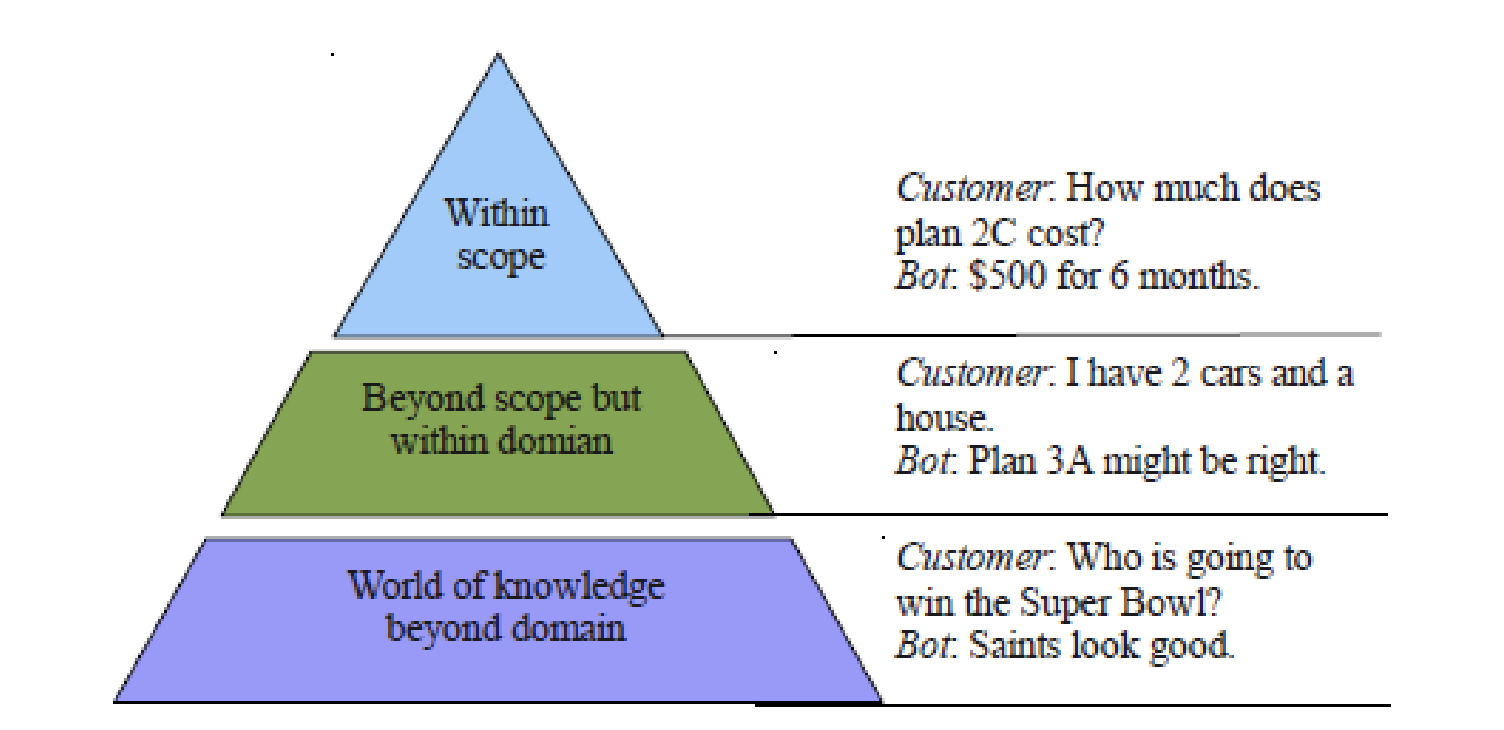
\includegraphics[width = 100mm]{conv-classes}
	\caption{Classes of Conversations: Within scope denoting specific conversations
within the domain, beyond scope denoting non-specific open-ended conversations
within the domain, and Beyond domain denoting conversations beyond the domain
being considered \cite{chakrabarti2015}.}
	\label{classes-of-conversations}
\end{figure}

Consider a snippet of conversation with a customer service chatter bot that helps customers solve account access issues. In this exchange, the customer is unable to login to an account, and seeks assistance \cite{chakrabarti2015}.
  \bigskip

{\fontfamily{cmss} \selectfont

  \color{red}
  \textbf{Chatter Bot}: Hello. How can I help you today ?
  \bigskip
  
  \color{blue}
  \textbf{Customer}: I am unable to login to my account. I forgot my password.
  \bigskip
  
  \color{red}
  \textbf{Chatter Bot}: Please click on the "Forgot Password" link. You will be emailed a link that will help you change your password.
  \bigskip
  
  \color{blue}
  \textbf{Customer}: I already tried that. That link takes me to a form to reset password. But it requires me to enter my Customer Relationship Number. I do not have this number.
  \bigskip
  
  \color{red}
  \textbf{Chatter Bot}: The Customer Relationship Number can be found in the "Account Information" tab when you log in to your account.
  \bigskip
  
  \color{blue}
  \textbf{Customer}: But I am unable to login to my account. I do not remember my password.
  \bigskip
  
  \color{red}
  \textbf{Chatter Bot}: Please click on the "Forgot Password" link. You will be emailed a link that will help you change your password.
  \bigskip
  
  \color{black}
}

To a human representative, it would be clear that this conversation is not helping address the customer’s issue. However, since chatter bots are programmed through pattern-template pairs, they are more suited for question-answer type exchanges, where there is a sequence of several question-answer pairs. They are unable to hold a longer conversation, understand the conversation, gauge whether the conversation is going in the desired direction, and act on it. In the above example, we expect the chatter bot to recognize the deadlock situation for the customer and to resolve it, or transfer the conversation to a human representative if the solution is beyond its programmatic capabilities.

It is clear from the example that the conversational performance of these chatter bots does not live up to what we would expect from a human customer service agent. Hence, there is clearly an opportunity to improve their conversational ability. In addition, since chatter bots cannot actually follow a longer conversation, they are also incapable of spotting opportunities in a conversation for providing unsolicited but pertinent information.




\chapter{Conversational Interfaces}
\label{cap:capitolo2}
% !TEX encoding = UTF-8
% !TEX TS-program = pdflatex
% !TEX root = ../Tesi.tex
% !TEX spellcheck = it-IT

%************************************************

%************************************************

Users' interactions with chatbots often mimic interactions between humans, but there are differences. In a study comparing human–human interactions to human– chatbot interactions, Hill et al. found that human–chatbot interactions tend to last longer than human–human interactions between strangers and involve shorter messages, less complicated vocabulary, and more profanity \cite{hill2015}.
Corti and Gillespie investigated whether users seek to repair misunderstandings in conversations with natural language user interfaces, which is important in any type of dialogue \cite{corti2016}. They found that, for chatbots perceived as human, users made more of an effort to repair misunderstandings than did users that perceived the chatbots as automated.
Several studies have investigated users’ experiences with chatbots. For example, Holtgraves et al. explored how users perceive chatbots’ personalities \cite{holtgraves2007}, and De Angeli et al. studied how the implied anthropomorphism of chatbots may elicit negative responses among users \cite{deangeli2001}. It may be important for chatbots to engage emotionally with users. A recent study by Xu et al. on customer service chatbots found that about 40\% of user requests to customer service are emotional rather than seeking specific information \cite{xu2017}. Without the ability to relate to these customers emotionally, a customer service chatbot risks failure.

\section {General} %%%%%%%%%%%%%%%%%%%%%%%%%%%%%%%%%%%%%%%%%%%

In their study, Tatai et al. \cite{tatai2003} compared implementations of chatbots and identified three main roles of chatbots, namely:

\begin{itemize}
\item Role of a Digital Assistant;
\item Role of an Information Provider;
\item Role of a General Chatbot
\end{itemize}

Examples of digital assistant chatbots are from IKEA, which was launched in 2005 and Niki.ai which helps you shop through chat. Chatbots can be used to improve the communication between doctor-patient (DP) and clinic-patient (CP). The researchers claim that using chatbots for this purpose (DP and CP communication) could reduce costs and time on routine operations \cite{abashev2017}. More implementations of chatbots are: credit score coach, personal stylist, food orderer, personal concierge, doctor, pension or finance advisor, teacher, newsreader, toy, accountant.
% * <siciliani.lu@gmail.com> 2018-04-06T16:19:46.424Z:
% 
% > 1
% ?
% 
% ^.

Chatbots can be found in different domains such as: customer service, e-commerce, insurance, healthcare, retail and more. 95\% of the respondents of a chatbot survey believed that the customer service domain is going to be ’the major beneficiary of chatbots'.

An example of a chatbot implementation in the financial field is K2 Bank. This chatbot checks your balance, your recent history of transactions and can make simple money transfers \cite{k2bot}.

Human-system dialogues consists of the inquirer (the user), looking for information, and the expert (system), providing information. There are two ways in which chatbots can converse with users. System-initiated chatbots, where the system leads the conversation, and user-initiated chatbots, where the user leads the conversation. Systems that contain both methods of initiation, are called mixed initiative systems \cite{hung2009}
% * <siciliani.lu@gmail.com> 2018-04-06T16:22:52.383Z:
% 
% > that
% in which
% 
% ^.
% * <siciliani.lu@gmail.com> 2018-04-06T16:21:01.367Z:
% 
% > dialogue
% "dialogues" (vedere poi le concordanze con i verbi successivi)
% 
% ^.

To understand how a conversational interface should be represented, it is important to investigate how human dialogues work. Quarteroni, et al. \cite{quarteroni2009} researched the aspects and issues related to human dialogues and they proposed a list of essential items for an interactive question answering system:
% * <siciliani.lu@gmail.com> 2018-04-06T16:24:16.002Z:
% 
% > question and answering
% question answering
% 
% ^.
% * <siciliani.lu@gmail.com> 2018-04-06T16:23:59.662Z:
% 
% > item
% items
% 
% ^.

\begin{itemize}
\item \textbf{Context Maintenance}: utilizing the context of the conversation to correctly interpret the user’s input. This is important for follow-up questions, or for clarification.
% * <siciliani.lu@gmail.com> 2018-04-06T16:24:44.243Z:
% 
% > utilising
% utilizing
% 
% ^.
\item \textbf{Utterance Understanding}: the detection of follow-up and clarification within the context of the previous conversation.
\item \textbf{Mixed Initiative}: the user should be able to take initiative within the conversation (by quitting, or asking questions).
\item \textbf{Follow-up Proposal}: meaning that the system motivates the user to give feedback on the answers that the system gives (if the user is satisfied or not). Until the user has achieved his or her goal.
\item \textbf{Natural Interaction}: covering and generating a variety of utterances to create a smooth conversation and to keep the dialogue active.
\end{itemize}

McTear \cite{mctear2016} reviewed key features of conversation in chapter 3 of his book on conversational interfaces. He describes that the following aspects are important when designing conversational interfaces:

\begin{itemize}
\item \textbf{Conversation as action}: meaning that utterances of users could be seen as actions that speakers carry out to achieve a goal.
\item \textbf{The structure of conversation}: regarding how utterances from a conversation relate to each other. Examples of ways to recognize structure in dialog acts can include adjacency pairs, exchanges, discourse segments and conversational games.
\item \textbf{Conversation as a joint activity}: describes how two parties take turns and reduce the risk of a miscommunication by using the grounding process in their conversation.
\item \textbf{Conversational repair}: a repairing process that can be initiated by one of the two parties in the conversation. Sometimes the speaker repairs his own utterances before the receiver has time to repair it.
\item \textbf{The language of conversation}: the tone of voice in a spoken text can be a way to convey additional information, such as emotions and affect. For example, when persons raise their voice when they are angry. For written text, emotions and affect can also be conveyed, for example by using emoticons or capital letters.
\end{itemize}

Incremental processing is an important process in human to human conversation. Incremental processing means that overlap occurs within a conversation. In human-machine interaction, a latency between turns is present. This is one reason why human-computer interaction can sometimes feel less natural than human to human interaction. Another benefit of incremental processing is that the dialog becomes more fluent and efficient \cite{mctear2016}. Google search applies incremental processing by completing the user’s query during typing and in Voice Search by showing the recognised words while the user is still speaking.




\section{Dialogue Management Strategy} %%%%%%%%%%%%%%%%%%%%%%%%%%

McTear \cite{mctear2016} describes that one of the core aspects of conversational interfaces is the design of the dialogue management strategy, in which the system’s conversational behaviour is defined. The design of dialogue management strategy was done manually in the past, but the research community has found ways to automate this process by training the model with real conversations. Two arising design strategies of dialogues in chatbots are the interaction strategy and the choice of a confirmation strategy. Automatic speech recognition is not always accurate, but by asking the user for confirmation or reprompt them, some errors could be avoided. Too many confirmation asking can also be annoying. There are three types of interaction strategies in chatbots, namely: user-initiated, system-initiated or mixed initiative. Limitations of user-initiated dialogues are errors in speech recognition and understanding, since users can say anything they want. The limitation of system-initiated dialogues, is that the user’s input is limited, but the advantage is that the interaction is more efficient. 

The advantage of a mixed-initiated dialogue is that the system can guide the user, but the user is also free to say anything he wants and take initiative, ask questions and introduce new topics. The limitations are that the system has to be technically advanced to keep track of his own structure/agenda, understand and answer the user’s utterances correctly and remember the relevant information said. Confirmation strategies are strategies to prevent errors in recognition and understanding of the user’s utterances. The disadvantage of using these confirmations is that it can make the interaction inefficient, repetitive and lengthy which can eventually lead to a frustrating user experience. 

A solution for these problems, is to create implicit confirmations. In this way, the user’s input is used in the next system’s output and extra information is added. To clarify the difference between implicit and explicit confirmation, we give the following example. When the user says the price of the house he wants to buy is \euro180.000, the system could say: "So the house you want to buy is \euro180.000 ?", which is an explicit confirmation. An implicit confirmation of the system would be: "So the house you want to buy costs \euro180.000. How much will an optional refurbishment add to the costs ?". A limitation of implicit confirmation strategy is that the user is responsible for correcting the system when it did not recognize the user’s utterances correctly \cite{mctear2016}



\section{Guidelines} %%%%%%%%%%%%%%%%%%%%%%%%%%%%%%%%%%%%%%%%%%%

\paragraph{Personality by design}
The chatbot personality is what gives the feeling of a natural conversation with an individual and comfort in the conversation. Designing the appropriate personality can increase the user experience and engagement with the bot. Personality is the tone the bot takes in a conversation. For example, if the bot is intended for e-commerce, then the bot personality should cover features, such as understanding the context of the conversation, is the user browsing or looking for specific information. Moreover, personality also includes knowing what the user might ask for and what the bot can’t offer. There is no one-size-fits-all approach when it comes to designing the correct conversation flow and currently there are no patterns that work for all cases. Most bots lack the structure to steer a conversation from the beginning to the end. Bots personality has to defines steps to guide user to learn and manage their intention. The bot should always be one step ahead of the user. For example, the bot should state which topics it covers when greeting the user, as below:
\bigskip

{\fontfamily{cmss} \selectfont

  \color{blue}
  \textbf{Bot}: I can help you to book a table, select menu and pay online..
  \bigskip
 
  \color{black}
}

This guiding is helpful and will result in one of the provided options being selected by the user. We need to understand what motivates us within a conversation and how can this be programmed into chatbots behaviour. Personality in chatbot is the new UX within conversational UIs \cite{fadhil2018}. Bot personality have to reflect the specific domain it is employing. For example, if we have a bot to take pizza orders, then one possible personality reflection could be that a significant number of people are asking for Pizza flavors not available. In this case, the bot has to provide clever responses that also progresses the conversation, instead of falling into a dead-end, as illustrated below:
\bigskip

{\fontfamily{cmss} \selectfont

  \color{red}
  \textbf{Chatter Bot}: You can select pizza pepperoni, pizza margherita and pizza with veggies. What is your choice?
  \bigskip
  
  \color{blue}
  \textbf{Customer}: I want pizza pepperoni
  \bigskip
  
  \color{red}
  \textbf{Chatter Bot}:  1 pizza pepperoni, cool, now tell me the size (small, medium, large)?
  \bigskip
  
  \color{black}
}


\paragraph{Flexibility in Response}
The bot should provide flexible values to various user requests. To illustrate, providing different error messages as response to the same question arose by the user. Moreover, the bot should cover irregular cases, such as a keyword related to another branch of the decision tree or a completely irrelevant keyword to the context. For instance, asking about a service before getting confirmation of success during a payment and causing early termination. If the user asks a random question or tricks the bot with unrelated questions, then it is critical that the bot doesn not repeat itself with a response such as:
\bigskip

{\fontfamily{cmss} \selectfont

  \color{red}
  \textbf{Chatter Bot}: Bot: Sorry I didn’t understand
  \bigskip
  
  \color{black}
}

If the bot continues to provide no information on alternate course of action, then the probability a user will leave the bot is very high. A best strategy is to play with multiple types of response or error messages and see what gets the best response from your user by focusing on a humorous or satirical approach to the problem. More importantly, provide different error messages for specific errors that occurs in a conversation \cite{fadhil2018}. If the error occurs when the user is asked to provide some information, such as their address, then the bot could respond:
\bigskip

{\fontfamily{cmss} \selectfont

  \color{red}
  \textbf{Chatter Bot}:  Sorry I’m still learning, try formatting your address 6500 Park Avenue, Hoboken, NJ 11211
  \bigskip
  
  \color{black}
}

\paragraph{Text vs Custom Buttons}
Users shouldn’t be placed in a situation where they have to guess the correct information required to proceed. Moreover, the bot should support a dictionary databased for synonyms so to yield the same result for vocabularies, such as "buy" and "purchase" or "client" and "customer". Custom keyboards or buttons permit a limited range of inputs and can save a bunch of typing. To illustrate, rather than asking end user to type “Yes” or “No” text, the bot can present them with two mutually exclusive buttons. Moreover, the bot can validate structured text link email address before sending. This way allows the bot to keep responses on track and sidestep the complications of parsing unpredictable plain text input \cite{khan2018}. They bot should never leave the user clueless in case of unrecognised questions and provide a fallback response to guide user as to what the next step might be. For example, provide the main topics from the content domain available. Rather than just using free text NLP communication with the bot, a proper UI should present options to the user to guide them through a decision making process. For instance, if the user is checking for a jacket, the interface can suggest a few of the company’s latest styles and similar items, as given below.
\bigskip

{\fontfamily{cmss} \selectfont

  \color{blue}
  \textbf{Customer}: I want to buy a snow jacket
  \bigskip
  
  \color{red}
  \textbf{Chatter Bot}: We have item1, item2, item3
  \bigskip
  
  \color{black}
}

\paragraph{Simplicity in Interaction}
Beyond the seemingly human aspect of communicating in the right tone and predicting and learning the user through a task, an additional reason CUI will work well in domains, such as healthcare is their simplicity. Conversational interfaces has to be bounded to particular subjects and follow a linear conversation routes \cite{bers1998}. Users often are looking for a service that finds them the answer with no extra effort. Therefore, individual designers should avoid complicated branching paths and shouldn't have to account for tricky failure cases. Moreover, utilizing auto-complete whenever possible and suggesting questions with the same wording are both effective to steer and inform users. This will shorten typing effort, since users can select one for the items in the auto-complete list \cite{khan2018}.

\paragraph{Conversation Flow}
Question and answer conversational interfaces are not the most effective way of getting answers from a bot, no matter how intelligent they are. For example, when ordering a food through a bot and when user isn't sure what to order, then they have to go through a conversation with the bot to figure out what to order. The conversation path becomes important, since it can help figure out how the conversation flow should be designed. Moreover, if the user can’t find answer to his question, it makes sense to add an option for the user to provide a feedback to save user question. The point is to prevent user from getting frustrated and provide a guidance instead of repeatedly saying "Sorry, I did not understand that"

\paragraph{Tasks and Duty Specifications}
Starting with rigid syntax, then introducing NLP is a best practice to start with when designing CUI \cite{fadhil2018}. The issue with NLP is that even if it supports complex conversation and gets the sentences right in most cases, it will fail in the remaining sentences in a very predictable way. Even if the bot provides fun error messages and smart responses to various user questions, this failing might lead to user frustration. NLP is perhaps the biggest bottleneck when designing CUIs. Humans always do spelling, grammar or typo mistakes. In addition, users often use slang and nuance to express something which can make any NLP based system to struggle. In fact, some services rely on employees to manage their conversation UI. NLP is effective in specific tasks, it is tedious to type and error prone. Therefore, focusing on creating a good UI is more important than a complex NLP. There are a number of ways in which NLP falls short of the requirements for a good UX by comparison with traditional UIs. For one thing, people are lazy and it feels easier to click a button, as we do on apps and websites, than typing out the whole sentence that the bot may will not understand. In addition, people easily fall into typo mistakes and the text they input may be full of grammar and spelling mistakes. This will result in user frustration with the bot in the long-term, since it can't understand their demands. Even worse, it may do the opposite of what it was asked for.


\paragraph{Empathy and Emotional State}
One of the pillar in CUI design patterns is to consider building an empathy with the user. All the design should be approached with empathy, in fact, many conversational interfaces integrate pauses, humans take a second to type an answer, so it makes sense to build a typing indicator for a bot. Addressing a social issue requires emotional sensitivity, a critical skill that bots are universally missing. Bots have to present some aspects of emotional state changes (fear, anger, sadness, etc.). In this regard, LawBot \cite{lawbot} which is a legal bot created by Cambridge University students to help users understand the complexities of the law and identify whether a crime has been committed. The bot is used to report sexual harassment, injuries and assaults, and property disputes. However, the bot relies on strict role based checklist to assess if a crime has been committed. If the user reports sexual harassment, and it doesn't fit within present criteria, the bot response with the following:
\bigskip

{\fontfamily{cmss} \selectfont

  \color{red}
  \textbf{Chatter Bot}:  I don’t think a sex offence was committed here. Say "Crime" for a list of what I can help you with.
  \bigskip
  
  \color{black}
}

Despite good intentions, the emotionally insensitive LawBot quickly dismisses sexual harassment if the harassment does not fit within a narrow set of legal technicalities. The results can be counterproductive and further discourage victims to speak up.


\paragraph{Keep Conversation Short}
Human-bot interaction should be short and precise \cite{fadhil2018}. Introducing a protracted back and forth conversation will make it feel laborious and hard to interact with the bot. Instead, bots have to serve specific tasks and intend for specific domains, in other words, personalized for a specific purposes. Unlike, graphic interface that defines rules for each interaction which often frustrate users, conversational interface has to be liberating in their familiarity.

\paragraph{Fully/Partially Automated}
Before introducing any functionalities into the bot, one should ask themselves whether a human will be better for the end user or a bot will deliver a more effective service. Bots are not to replace what humans are good at, rather they should improve what humans are slow at. As much advanced in Machine Learning and AI are going to help with automation where it makes sense, it is also true that we will absolutely need a human being in the loop to create the right end-to-end customer experience. It is a good practice to start with real humans, doing 100\% of the work, then, introduce role-based hierarchical tree. Only after that, introducing NLP to automate the 10\% of the most common tasks \cite{fadhil2018}. As an example, introducing NLP to the most frequently asked questions or just for the on-boarding. At later stages, especially when we have enough dialogue data, then we can move up and introduce more automation and intelligent machine learning techniques. This strategy applies when the value of the bot is in the human expert \cite{khan2018}.

\paragraph{Provide a Way Out}
Humans make mistakes, therefore, bot users should always be able to start over, make changes, or completely escape when a mistake occurs. Sometimes, humans get into a conversation without a correct established base facts. However, when it becomes clear that the other party is lost, we start over or stop the conversation, bots should do the same.\\

{\fontfamily{cmss} \selectfont
 
  \color{red}
  \textbf{Chatter Bot}: Would you like to order pizza? 
  \bigskip
  
  \color{blue}
  \textbf{Customer}: I am not sure what to eat tonight 
  \bigskip
  
  \color{red}
  \textbf{Chatter Bot}: How about a list of available restaurants to order from?
  
  \color{black}
}



% \section{Personalization}

% Chapter 2 discusses several studies in the literature that try to solve problems related to the task in this dissertation. These studies can be roughly classified into three groups: the syntactic approach, the stochastic approach, and the semantic approach. Stochastic approaches use statistical frameworks like Bayesian theory, Hidden Markov models, and n-gram modeling to construct individual sentences. Syntactic approaches use techniques from natural language processing and computational linguistics to parse and model grammatical constructs of conversations. Semantic approaches use models of meaning from a knowledge structure to drive sentence analysis and construction. The most representative studies in each approach are described here in detail. As with most research, studies under all three umbrellas heavily leverage ideas from each other.




% \section{The Stochastic Approach}

% The earliest formal architecture designed for conversations was the Bayesian Receptionist at Microsoft Inc \cite{horvitz2000}. The system maintained a domain of dialogues about goals typically handled by receptionists at the front desks of the buildings on the Microsoft corporate campus. The system employed a set of Bayesian user models to interpret the goals of speakers given evidence gleaned from a natural language parse of their utterances. Beyond linguistic features, the domain models took contextual evidence into consideration, including visual findings.

% The 3-level task abstraction hierarchy was the key feature of the system. Each level modeled a different level of abstraction. Level 0, the highest level of abstraction, modeled the task of discriminating the high-level goal of the user, given initial observations and an initial utterance. Level 1, the next lower level of abstraction, modeled the refinement of the high-level goals into more specific goals. Level 2, the lowest level of abstraction, modeled additional conditions for specific situational cases. Levels more detailed than the highest level included an additional state representing the proposition that the current level is inappropriate.

% Inference about the belief assigned to each state was used to control backtracking in conversation. Decomposition of a user’s goals into several levels of detail allowed for guiding conversation on a natural path of convergence toward shared understanding at progressively greater levels of detail. Multiple levels also allowed for the establishment of common ground \cite{clark1996} about uncertainties at each level. It
% also allowed conversation regarding comprehension of misunderstandings before progressing
% to the next level of detail.

% In the Microsoft system, users could be directed, as part of a natural dialog about their goals, to implicitly or explicitly confirm or disconfirm misunderstanding at each level. This lead to reduction of uncertainty to some tolerable level before progressing to the next level. The limitation of this model was that it scaled poorly. It was unable to model any conversation beyond asking for direction. But, it also introduced some important ideas about leveraging probabilistic methods for inferencing at different levels of abstraction.

% Paek and Horovitz \cite{paek2000} then demonstrated how conversations could be modeled as an inference and decision making problem under uncertainty. They designed Quartet, a task independent, multimodal architecture for supporting robust continuous spoken dialog. Their model had four levels of independent analysis. A channel level established mere exchange of utterances. A signal level established intent. An intention level which modeled semantics of the conversation. Finally a conversation level, modeled a tangible activity or behavior based on the conversation.

% The Paek and Horovitz model also included learning the parameters of the inference model using an expectation maximization type algorithm. The architecture maintained a probability distribution function over communication failure modes, and minimized this failure function at each level. One limitation of this model was that it relied on ad hoc policies to deal with failures at each level, and these policies had to be designed independently for every class of conversations.

% Li and Ji \cite{li2005} used a probabilistic framework based on dynamic Bayesian networks to model an user’s affective states. Although they model general behaviors, not conversations, they were one of the earlier works that introduced the concept of state-based modeling for human behavior. They systematically modeled the uncertainty, dynamics, and different types of knowledge associated with user affective state using DBNs. They demonstrated an information-theoretic mechanism to perform active behavior learning. They also demonstrated user affective state inference in a timely and efficient manner, and proposed information-theoretic criteria to optimally determine when and what assistance to provide to maximize the chance for returning the user to its normal state while minimizing interference with the user’s workload and annoyance. The main contribution lies in the integration of the proposed active sensing mechanism into the DBN-based framework for user state inference and user assistance.

% Mishne et al. \cite{mishne2005} introduced a novel method of estimating the domain-specific importance of conversation fragments from call center telephone calls, based on divergence of corpus statistics. The main novelty of their system was a method for identifying the domain-specific importance levels of fragments in the call, and usage of this method for retrieving possible solutions to the problem presented in the conversation, and for detecting abuse of the call-center resources. A simple way of estimating the significance level of a fragment of a call is to estimate the significance level of each word in the fragment and combine these individual values. In most text analysis systems, the significance of words is inversely related to their frequency. The more common a word is, the less significance it has. Estimating the significance level of a word requires an evaluation of how characteristic the word is to a specific domain, compared to other domains. Rather than global significance, they actually estimated domain-specific word significance (and hence, domain-specific fragment significance). They also used manually transcribed data for validating their results.

% Ozyurt and Kose \cite{ozyurt2010} used Naive Bayes, k-nearest neighbor, and support vector machines to automatically mine chat conversation topics in Turkish language call center conversations. Threads and endings of the topics were determined by making analysis at the sentence level rather than the conversation level. They used a Dirichlet prior distribution to initially model the distribution of topics across each sentence, and then support vector machines to learn their final distributions.

% Douglas et al. \cite{douglas2005} designed a tool for mining customer care chats for news items of importance. Relevant business and dialog features were extracted from the speech logs of caller-system interactions and tracked by a trend analysis algorithm. Features that moved outside their expected bounds on a given day generated headlines as part of a web site generated completely automatically from each day’s logs.






% \section{The Syntactic Approach}

% Many researchers have tried to solve the specific problem of mining and modeling conversations in the context of customer service agents using a variety of cookbook techniques.

% Takeuchi et al. \cite{takeuchi2007}, designed a method to analyze transcripts of conversations between customers and human agents at a service center. Their aim was to obtain actionable insights from the conversations to improve agent performance using a three step approach. First, they segmented the call into logical parts. Next they extracted relevant phrases within different segments. Finally, they performed 2-dimensional association analysis to identify actionable trends. They used real conversational data from a service center to identify specific actions by agents that resulted in positive outcomes. They showed that associations between agent utterances and outcomes could be found by segmenting the calls and aggregating phrases within the call segments. In particular they analyzed calls to answer some of the key questions faced by question-answers with the objective of improving agent productivity.

% In subsequent work, Takeuchi et al. \cite{takeuchi2007conversation} argued that the language patterns in the final stages of electronic negotiations are more indicative of the outcomes, whereas in face-to-face negotiations the initial stages of the negotiations are more useful for predicting the outcome.

% Roy and Venkata. \cite{roy2006} used unsupervised learning algorithms to generate domain models automatically from telephone conversation transcriptions. Their domain model was comprised primarily of a topic taxonomy where every node was characterized by topics, typical questions and answers, typical actions, and call statistics. This hierarchical domain model contained summarized topic specific details for topics of different granularity. However they did not use any semantic features in their taxonomy.





% \section{The Semantic Approach}

% Chai et al. \cite{chai2005} introduced a fine-grained semantic model that characterized the meanings of user inputs and the overall conversation from multiple dimensions for unified multi-modal input understanding. They also realized discourse interpretation through an integrated interpretation approach that identified the semantics of user inputs and the overall conversation using a wide variety of contexts. They achieved a 90\% accuracy in recognizing the meaning of user input. However the interpretation rules were manually contracted for the models. The rules had to handcrafted each time for different domains, and as a result scaled poorly.

% Mehta and Corradini \cite{mehta2007} demonstrated the representational power of ontologies for a spoken dialog system. Their system focused on the categorization of ontological resources in to domain independent, and domain specific components. These domains were leveraged to augment the agents conversational capabilities and enhance the systems reusability across conversational domains. They leveraged Google directory categorization for a semi-automatic understanding of a user utterance on general purpose topics like movies and games.



\chapter{Conversational Interfaces in Finance}
\label{cap:capitolo3}
% !TEX encoding = UTF-8
% !TEX TS-program = pdflatex
% !TEX root = ../Tesi.tex
% !TEX spellcheck = it-IT

%************************************************

%************************************************

\section{QA FAQ Customer Support}

\section{Functionalities}



















The way we have been interacting with our banks and insurance companies has been changing drastically \cite{khan2018}. The BFSI sector is a pioneer in the adoption of new technology. Previously, we either had to visit a bank branch or contact our relationship manager even to request a new checkbook. Today, all these services are just a click away on a web site or mobile app. The next wave of technology adoption has already started by some of the largest banks and insurance companies in the world, wherein they are adopting chatbots for specific use cases and deploying them on a large scale. 







\chapter{Critical analysis}
\label{cap:capitolo4}
% !TEX encoding = UTF-8
% !TEX TS-program = pdflatex
% !TEX root = ../Tesi.tex
% !TEX spellcheck = it-IT

%************************************************

%************************************************


Consumers are increasingly relying on messaging apps for all types of communication weather it may be personal or business.
Shifting the way we interact with technology from commands to conversations will reshape digital experiences. It will enable organizations to reduce operational costs and identify new revenue opportunities and business models. Sometimes customers have some doubts during online payments and at that time they need someone to sort out their doubts, and this conversation can be easily fulfilled by messaging apps. Increasingly customers are using messaging applications and online chatting application to find and select products and services and to complete the payment process, all without having to mail or even to visit the particular brand website. 

The culture of online internet marketing is increasing day by day and this culture is being accepted by the customers. In favor to promote this new culture the messaging apps are also covering the gap and building a common platform where the customers and companies get the best way of conversation to get their deals done and get some profitable outcome. Everyone knows how to use messaging platforms, so there is nothing to relearn. Instead of having to switch to a web page to complete a payment, conversational commerce lets you transact right inside the messaging interface. This makes for a smoother, more effortless user and customer experience \cite{piyush2016}. Why should one build a bots ? Messaging platforms are the new browsers and bots are the new websites. This is a great opportunity to connect with your audience in a one on one and yet scalable manner.

Conversational agents have great business potential for several reasons. They provide a safe platform for transaction and a natural way of online marketing. Conversational commerce has a lot of future scope and it will grow the business environment of marketing. It gives you the platform for direct interaction between the customer and the company personas.

Conversational agents have brought a new revolution in field of business and marketing, It gives a better experience to both the seller as well as customers also and it saves time as well as money. Nowadays about days 52\% of the population prefer online shopping rather than mall or shop visit purchasing \cite{piyush2016}.

It's all about giving customers a reliable and easy platform to save their time and to make them feel better. It has been found that there are more than 2 billion Smartphone users in the world and they increasingly day by day are getting addicted to Smartphone and can't spend much time without them. And no wonder there is a growing interest in conversational agents \cite{piyush2016}.


% \chapter{Critical analysis}
% \input{Capitoli/Conclusioni}


\bibliographystyle{plain}
\bibliography{Bibliografia}

\end{document}
